% =============================================================================
\section{Bonding Curve Graduation}
\label{sec:bonding-curve}
% =============================================================================

This section formalizes the quadratic bonding curve used for agent token
issuance, derives the cost function, proves key properties, specifies the
graduation mechanism, and compares the quadratic form against alternative curve
shapes.

\subsection{Quadratic Pricing Function}
\label{subsec:pricing}

\begin{definition}[Bonding Curve Price]
\label{def:bc-price}
Let $q \geq 0$ denote the cumulative quantity of agent tokens sold. The
instantaneous price is defined by the affine function:
\begin{equation}
  P(q) = B + S \cdot q
  \label{eq:price-function}
\end{equation}
where $B > 0$ is the base price (in CORTEX per agent token) and $S > 0$ is
the slope parameter.
\end{definition}

The base price $B$ sets a nonzero floor that prevents zero-cost acquisition of
the first tokens, while the slope $S$ determines the rate at which marginal
price increases with cumulative supply. Both parameters are set at agent
creation time and are immutable thereafter.

\subsection{Cost Function}
\label{subsec:cost}

A buyer purchasing $n$ tokens when the current cumulative supply is $s$ pays
the integral of the price function over the interval $[s, s+n]$:

\begin{equation}
  C(s, n) = \int_{s}^{s+n} P(q) \, dq = \int_{s}^{s+n} (B + Sq) \, dq
  \label{eq:cost-integral}
\end{equation}

Evaluating:
\begin{align}
  C(s, n) &= \left[ Bq + \frac{S q^2}{2} \right]_{s}^{s+n} \notag \\
  &= B(s+n) + \frac{S(s+n)^2}{2} - Bs - \frac{Ss^2}{2} \notag \\
  &= Bn + \frac{S}{2}\left[(s+n)^2 - s^2\right] \notag \\
  &= Bn + \frac{S}{2}(2sn + n^2) \notag \\
  &= n \cdot B + \frac{S(2sn + n^2)}{2}
  \label{eq:cost-closed}
\end{align}

The average price per token for this purchase is:
\begin{equation}
  \bar{P}(s, n) = \frac{C(s, n)}{n} = B + S\left(s + \frac{n}{2}\right)
  \label{eq:avg-price}
\end{equation}

which equals the price at the midpoint of the interval $[s, s+n]$, a
consequence of the linearity of $P(q)$.

\subsection{Monotonicity and Convexity}
\label{subsec:monotonicity}

\begin{proposition}[Monotonicity and Convexity]
\label{prop:monotonicity}
The cost function $C(s, n)$ satisfies:
\begin{enumerate}
  \item[(i)] \textbf{Monotonicity in $s$:} For fixed $n > 0$,
    $\partial C / \partial s > 0$.
  \item[(ii)] \textbf{Monotonicity in $n$:} For fixed $s \geq 0$,
    $\partial C / \partial n > 0$.
  \item[(iii)] \textbf{Convexity in $n$:} For fixed $s \geq 0$,
    $\partial^2 C / \partial n^2 > 0$.
\end{enumerate}
\end{proposition}

\begin{proof}
From Equation~\eqref{eq:cost-closed}:
\begin{align}
  \frac{\partial C}{\partial s} &= Sn > 0 \quad \text{since } S, n > 0. \label{eq:dc-ds} \\
  \frac{\partial C}{\partial n} &= B + S(s + n) = P(s+n) > 0 \quad \text{since } B, S > 0. \label{eq:dc-dn} \\
  \frac{\partial^2 C}{\partial n^2} &= S > 0. \label{eq:d2c-dn2}
\end{align}
Properties (i)--(iii) follow directly. \qed
\end{proof}

\begin{remark}
Property (iii) implies that the marginal cost of each additional token is
strictly increasing. This creates a natural scarcity premium: later buyers
pay more per token than earlier buyers, which (a)~rewards early price
discovery and (b)~discourages large single-transaction accumulation.
\end{remark}

\subsection{Graduation Mechanism}
\label{subsec:graduation}

\begin{definition}[Graduation]
\label{def:graduation}
An agent token \emph{graduates} when its bonding curve accumulates a total of
$G$ CORTEX in proceeds, where $G = 50{,}000$ CORTEX is the graduation
threshold. At graduation, the following atomic transaction group executes:
\begin{enumerate}
  \item The bonding curve is frozen (no further buys or sells).
  \item The accumulated CORTEX and remaining agent tokens form an LP pair on
    Tinyman.
  \item The LP tokens are transferred to a LogicSig account that enforces a
    10-year lock (Section~\ref{sec:security}).
  \item A graduation bonus is distributed: 50\% to the creator, 30\% to
    early buyers (pro-rata by purchase timestamp), and 20\% is burned.
\end{enumerate}
\end{definition}

The graduation threshold $G$ is a governance-adjustable parameter
(Section~\ref{sec:governance}). The atomic execution via Algorand transaction
groups ensures that no partial state transitions can occur---either the full
graduation completes or the bonding curve remains active.

\subsubsection{LP Lock via LogicSig}

The LP tokens are sent to an Algorand LogicSig account whose compiled program
enforces:

\begin{enumerate}
  \item No transactions are permitted until $t_{\text{graduation}} + 10
    \text{ years}$ (encoded as a round number based on 3.3-second block
    times).
  \item After the lock expires, only the AgentFactory contract can initiate
    withdrawal.
  \item The LogicSig program is stateless and immutable---once deployed, its
    logic cannot be altered.
\end{enumerate}

This provides a strictly stronger guarantee than EVM-based LP locks that rely
on time-lock contracts with potential admin keys.

\subsection{Graduation Bonus Distribution}
\label{subsec:grad-bonus}

Let $G_{\text{bonus}}$ denote the graduation bonus pool (a fixed percentage of
bonding curve proceeds designated for distribution). The allocation is:

\begin{equation}
  G_{\text{bonus}} = G_{\text{creator}} + G_{\text{early}} + G_{\text{burn}}
  \label{eq:grad-bonus}
\end{equation}

with $G_{\text{creator}} = 0.5 \cdot G_{\text{bonus}}$, $G_{\text{early}} =
0.3 \cdot G_{\text{bonus}}$, and $G_{\text{burn}} = 0.2 \cdot G_{\text{bonus}}$.

Early buyer shares are computed pro-rata by inverse purchase time:
\begin{equation}
  \text{share}_i = \frac{n_i \cdot (t_{\text{grad}} - t_i)^{-1}}{\sum_j n_j \cdot (t_{\text{grad}} - t_j)^{-1}}
  \label{eq:early-share}
\end{equation}
where $n_i$ is the number of tokens purchased by buyer $i$ at time $t_i$, and
$t_{\text{grad}}$ is the graduation timestamp. This weights earlier purchases
more heavily, rewarding participants who provided initial price discovery
capital.

\subsection{Comparison of Curve Shapes}
\label{subsec:curve-comparison}

\begin{theorem}[Quadratic vs.\ Linear vs.\ Exponential Curves]
\label{thm:curve-comparison}
Consider three bonding curve families parameterized to produce identical total
cost at a reference supply $q^*$:
\begin{align}
  P_{\text{lin}}(q) &= B_1 \quad \text{(constant/linear cost)} \label{eq:linear} \\
  P_{\text{quad}}(q) &= B_2 + S_2 q \quad \text{(quadratic cost)} \label{eq:quadratic} \\
  P_{\text{exp}}(q) &= B_3 e^{\alpha q} \quad \text{(exponential cost)} \label{eq:exponential}
\end{align}
Then for any $q > q^*$:
\begin{enumerate}
  \item[(i)] The exponential curve produces the highest marginal price:
    $P_{\text{exp}}(q) > P_{\text{quad}}(q) > P_{\text{lin}}(q)$.
  \item[(ii)] The quadratic curve maximizes the ratio of early-buyer surplus
    to late-buyer cost:
    \begin{equation}
      \frac{P_{\text{quad}}(q^*) - P_{\text{quad}}(0)}{P_{\text{quad}}(q) - P_{\text{quad}}(q^*)}
      > \frac{P_{\text{exp}}(q^*) - P_{\text{exp}}(0)}{P_{\text{exp}}(q) - P_{\text{exp}}(q^*)}
      \label{eq:surplus-ratio}
    \end{equation}
    for sufficiently large $q$.
  \item[(iii)] The quadratic curve uniquely satisfies both
    \emph{accessibility} (finite cost at all $q$) and
    \emph{scarcity} ($P'(q) > 0$, $P''(q) = 0$, linear price growth).
\end{enumerate}
\end{theorem}

The proof is provided in Appendix~\ref{app:proofs}. The key insight is that
the quadratic curve (linear price) occupies a Goldilocks position: it provides
meaningful scarcity premium (unlike the flat curve) without the explosive price
growth that makes the exponential curve inaccessible to later participants
(which concentrates value among insiders and reduces long-term liquidity depth).

\begin{figure}[H]
\centering
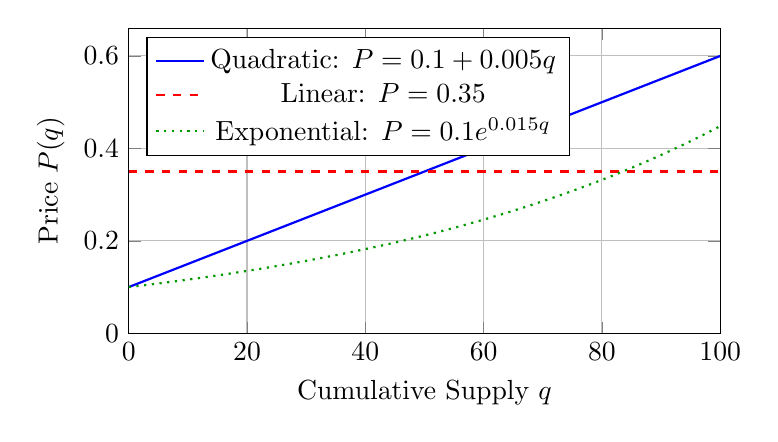
\begin{tikzpicture}
\begin{axis}[
  width=0.75\textwidth, height=0.45\textwidth,
  xlabel={Cumulative Supply $q$},
  ylabel={Price $P(q)$},
  legend pos=north west,
  grid=major,
  xmin=0, xmax=100,
  ymin=0,
]
\addplot[blue, thick, domain=0:100, samples=100] {0.1 + 0.005*x};
\addlegendentry{Quadratic: $P = 0.1 + 0.005q$}
\addplot[red, thick, dashed, domain=0:100, samples=100] {0.35};
\addlegendentry{Linear: $P = 0.35$}
\addplot[green!60!black, thick, dotted, domain=0:100, samples=100] {0.1*exp(0.015*x)};
\addlegendentry{Exponential: $P = 0.1 e^{0.015q}$}
\end{axis}
\end{tikzpicture}
\caption{Comparison of bonding curve price functions. The quadratic (linear
price) curve provides moderate scarcity premium while maintaining accessibility.
The exponential curve becomes prohibitively expensive; the constant curve
offers no scarcity incentive.}
\label{fig:curve-comparison-inline}
\end{figure}
